\part{Contribution: Conception and Design}

\chapter{Requirements Specification and Design}
\label{chap:requirements_design}

\section{Introduction}

This chapter specifies the functional and non-functional requirements of the Agrio platform and presents the main design diagrams used to guide the implementation. The requirements are derived from the literature gaps identified in Chapter~\ref{chap:scientific_positioning}, the project objectives, the implemented backend APIs, the PostgreSQL schema, the MQTT payloads, the dashboard and mobile workflows, and the actuator-control workflow. The objective is to describe what the system must do before presenting how the implementation is organized.

\section{System objectives}

The main objective of Agrio is to support intelligent irrigation decisions through a Digital Twin of a monitored agricultural zone. The system must receive sensor data from the physical prototype, store it, update the virtual state, predict irrigation need, simulate scenarios, request explainable MAS decision support, generate recommendations, display results to the user, and control the pump when a decision is validated or manually triggered.

The system must also remain demonstrable and maintainable. It should expose clear API endpoints, store data in a structured schema, separate the ML service from the backend, provide a dashboard for testing and operation, and support deployment through Docker Compose. These objectives keep the contribution realistic: the thesis targets a supervised prototype rather than a production-grade irrigation optimizer.

\section{Actors}

The main human actors are the farmer/operator and the administrator/agronomist. The farmer monitors the dashboard, checks zone conditions, reviews recommendations, validates decisions, schedules irrigation, and manually controls the pump if needed. The administrator or agronomist manages farms, plots, zones, sensors, soil profiles, crops, and system configuration. External technical actors include the MQTT sensor station, WeMos actuator, ML service, MAS service, weather API, and PostgreSQL database.

\section{Functional requirements}
\label{sec:functional_requirements}

Functional requirements describe the behavior expected from the platform. In Agrio, these requirements are derived from the research gap, the need for a complete Digital Twin loop, and the implemented artifacts of the system. The backend APIs define how users, zones, sensor data, predictions, simulations, recommendations, schedules, and device-control actions are exposed. The database schema defines which entities must be persisted. The MQTT payloads define how physical measurements, actuator commands, and WeMos feedback enter or leave the software system. The dashboard and mobile workflows define what the user must be able to monitor and validate.

Table~\ref{tab:functional_requirements} summarizes the functional requirements derived from the objectives described in Section~\ref{sec:functional_requirements}. The table is organized from acquisition to traceability so that it follows the complete irrigation workflow: physical measurement, ingestion, persistence, Digital Twin synchronization, prediction, simulation, MAS evidence generation, recommendation, validation, scheduling, actuation, feedback, and visualization.

\begin{footnotesize}
\setlength{\tabcolsep}{2pt}
\renewcommand{\arraystretch}{1.12}
\begin{longtable}{@{}p{0.07\textwidth}p{0.18\textwidth}p{0.31\textwidth}p{0.18\textwidth}p{0.18\textwidth}@{}}
\caption{Detailed functional requirements of the Agrio platform}
\label{tab:functional_requirements}\\
\toprule
ID & Requirement & Description & Main actor/component & Related workflow \\
\midrule
\endfirsthead
\toprule
ID & Requirement & Description & Main actor/component & Related workflow \\
\midrule
\endhead
FR1 & Receive MQTT sensor payloads & Receive structured sensor and environmental measurements from the field gateway through MQTT. & Raspberry Pi gateway, backend subscriber & Sensor ingestion \\
FR2 & Validate and normalize measurements & Parse JSON, validate required fields, convert units, normalize aliases, and reject unusable payloads. & Backend parser & Data preparation \\
FR3 & Map device and zone & Resolve the physical device and management zone associated with each payload. & Backend mapping service & Context resolution \\
FR4 & Persist sensor and weather records & Store timestamped sensor readings and weather records in PostgreSQL. & Backend, database & Persistence \\
FR5 & Evaluate sensor freshness and health & Check last-seen timestamps and device status to detect stale or missing data. & Backend health service & Monitoring \\
FR6 & Update Digital Twin zone state & Synchronize the virtual zone state from the latest sensor, weather, and actuator information. & Digital Twin service & State synchronization \\
FR7 & Store state history & Append state snapshots so that virtual-state evolution can be audited. & Digital Twin service, database & Historical trace \\
FR8 & Call ML service for prediction & Build the feature payload and request irrigation predictions from the separated Random Forest service. & Backend, ML service & Prediction \\
FR9 & Store prediction results & Persist irrigation need, suggested hour, confidence values, and fallback status when applicable. & Backend, database & Decision trace \\
FR10 & Run what-if simulation & Compare future moisture evolution under no-irrigation and irrigation scenarios. & Simulation service & Scenario analysis \\
FR11 & Generate base irrigation recommendations & Convert state, prediction, simulation, forecast context, and rules into user-readable advice. & Recommendation engine & Decision support \\
FR12 & Request MAS decision support & Send field context to the MAS service with \texttt{device\_id}, location, crop type, farmer note, optional zone, target moisture range, and irrigation duration. & Backend/frontend, MAS service & Explainable decision request \\
FR13 & Generate multi-agent evidence & Produce structured evidence blocks for Digital Twin state, ML prediction, weather, agronomy, water balance, and safety. & MAS agents & Evidence generation \\
FR14 & Fuse evidence with safety priority & Combine evidence using safety-aware priority so deterministic safety rules can block or redirect direct irrigation. & Coordinator Agent, Safety Rule Agent & Decision fusion \\
FR15 & Return farmer-friendly explanation & Return the final decision, confidence, risk level, suggested hour, duration, explanation, evidence, and warnings. & Explanation Agent, MAS API & Explainability \\
FR16 & Support human validation & Allow the user to accept, reject, or keep recommendations pending before physical execution. & Farmer/operator, dashboard & Supervision \\
FR17 & Create irrigation schedules & Store validated or user-defined irrigation events with planned start time and duration. & Scheduler workflow & Planning \\
FR18 & Execute scheduled irrigation & Detect due events and trigger the appropriate control workflow. & Irrigation scheduler & Scheduled control \\
FR19 & Publish actuator commands & Send pump-control commands to the WeMos actuator through MQTT. & Backend device-control service & Actuation \\
FR20 & Receive WeMos feedback & Receive status messages from the actuator and record whether the physical state changed. & WeMos actuator, backend & Feedback \\
FR21 & Display dashboard overview & Present current state, charts, predictions, recommendations, forecasts, schedules, MAS evidence, and device status. & Next.js dashboard & User monitoring \\
FR22 & Provide mobile access & Allow prototype/mobile testing of the same monitoring and control workflows. & Flutter application & Mobile operation \\
FR23 & Generate weather-aware forecast & Store and expose forecast context used by planning and recommendation workflows. & Forecast service, weather API & Forecasting \\
FR24 & Maintain traceability from measurement to action & Preserve links between readings, states, predictions, MAS decisions, recommendations, events, commands, and feedback. & Database, backend services & Audit trail \\
\bottomrule
\end{longtable}
\end{footnotesize}

These requirements cover the full Digital Twin loop because they begin with physical measurements and end with physical feedback after a command. They also connect directly to the design diagrams in this chapter: the use-case diagram identifies actors, the activity and sequence diagrams show runtime behavior, and the domain diagrams define the data structures that support traceability. Chapter~\ref{chap:backend_database_iot} explains how the backend and database implement these requirements.

\section{Non-functional requirements}

Non-functional requirements describe quality constraints. The system must be modular, maintainable, reproducible, and observable. It must support near-real-time dashboard updates, reliable message parsing, safe actuation, clear separation between simulation and physical control, and extensibility toward more zones and crops. The prototype also requires usability because the dashboard is central to decision support.

\begin{footnotesize}
\setlength{\tabcolsep}{2pt}
\begin{longtable}{@{}p{0.12\textwidth}p{0.25\textwidth}p{0.48\textwidth}@{}}
\caption{Non-functional requirements}\\
\label{tab:non_functional_requirements}\\
\toprule
ID & Requirement & Design implication \\
\midrule
\endfirsthead
\toprule
ID & Requirement & Design implication \\
\midrule
\endhead
NFR1 & Modularity & Separate backend, ML service, MAS service, frontend, scheduler, MQTT communication, and database responsibilities. \\
NFR2 & Traceability & Persist raw readings, states, predictions, recommendations, commands, and feedback. \\
NFR3 & Safety & Separate simulation from physical actuation, apply deterministic safety rules before direct irrigation, and preserve human validation for supervised actions. \\
NFR4 & Usability & Provide readable dashboard cards, charts, explanations, recommendations, and manual controls. \\
NFR5 & Reproducibility & Use Docker Compose and environment variables for local deployment. \\
NFR6 & Extensibility & Model farms, plots, zones, sensors, and device mappings so the prototype can grow. \\
NFR7 & Observability & Expose health/status information, logs, and database records useful during demonstrations. \\
NFR8 & Performance & Support near-real-time polling and fast ML inference for prototype operation. \\
NFR9 & Explainability & Expose final MAS decisions with confidence, risk level, evidence blocks, warnings, and farmer-friendly explanations. \\
NFR10 & Graceful degradation & Continue safely when ML, weather, or MAS evidence is incomplete by using deterministic fallbacks and conservative decisions. \\
\bottomrule
\end{longtable}
\end{footnotesize}

\section{Constraints}

The current system is constrained by the laboratory prototype, limited long-term field data, and available hardware. It is designed for controlled demonstration rather than immediate production deployment. The platform prioritizes functionality, integration, and traceability over advanced cybersecurity and large-scale distributed deployment. These constraints are documented to maintain academic transparency.

\section{Use-case model}

The use-case diagram represents the interaction between the farmer, administrator, IoT sensor station, WeMos actuator, ML service, and weather API. It includes monitoring, simulation, recommendation validation, manual command, forecast generation, data ingestion, sensor health evaluation, and ML prediction.

\begin{figure}[H]
    \centering
    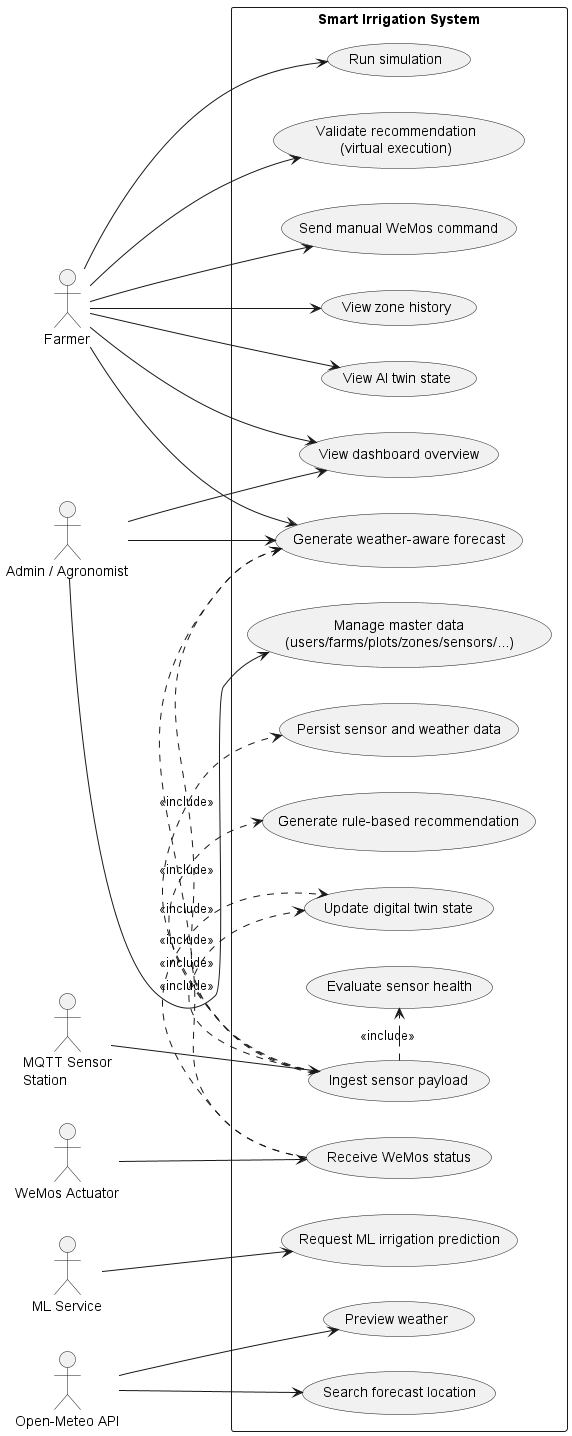
\includegraphics[width=\textwidth,height=0.85\textheight,keepaspectratio]{figures/chapter_05/fig_5-1.png}
    \caption{Use-case diagram of the proposed Digital Twin smart irrigation system.}
    \label{fig:5-1-use-case-diagram-of-the-proposed-digital-twin-smart-irrigation-sys}
\end{figure}

\noindent\textbf{Update note:} this use-case diagram should later be updated to show the MAS service as an external decision-support component used by the dashboard, backend, or final integration path.

\section{Activity workflow}

The activity workflow begins when the backend receives an MQTT sensor payload. The system validates and normalizes the payload, resolves the zone, creates missing sensor mappings if needed, inserts weather records and sensor readings, evaluates sensor health, updates the zone state, calls the ML service, stores predictions, appends state history, and exposes the updated state to the dashboard. If irrigation is required, the system waits for user confirmation. Validation can create a recommendation record and irrigation event, while manual device commands publish MQTT commands to the WeMos actuator.

\begin{figure}[H]
    \centering
    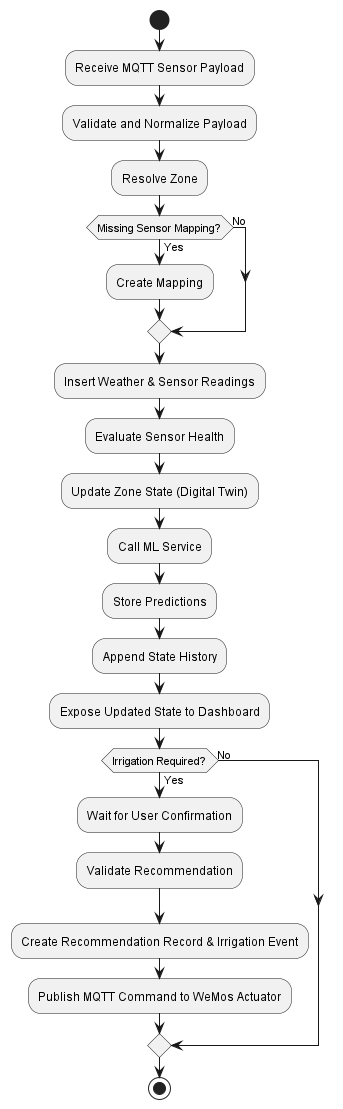
\includegraphics[width=\textwidth,height=0.85\textheight,keepaspectratio]{figures/chapter_05/fig_5-2.png}
    \caption{Activity diagram of sensor ingestion, Digital Twin update, AI decision-making, and pump control.}
    \label{fig:5-2-activity-diagram-of-sensor-ingestion-digital-twin-update-ai-decisi}
\end{figure}

\noindent\textbf{Update note:} this activity diagram should later be redrawn to include the MAS decision request after Digital Twin, ML, weather, and simulation context are available.

In the updated decision workflow, MAS fits between context preparation and final human validation. The Digital Twin state, ML prediction, weather context, target moisture range, selected duration, and farmer text note are sent to the MAS service. The MAS then returns a safe decision with evidence, warnings, confidence, risk level, recommended duration, and a farmer-friendly explanation. The user can inspect this output before validating a recommendation, scheduling an event, or keeping the pump off.

The sequence-level view in Figure~\ref{fig:runtime_sequence_design} complements the activity diagram by showing the order of interactions between the sensor station, MQTT broker, backend subscriber, parser, database, real-time pipeline, ML service, dashboard, device-control service, WeMos actuator, and status feedback.

\begin{figure}[H]
    \centering
    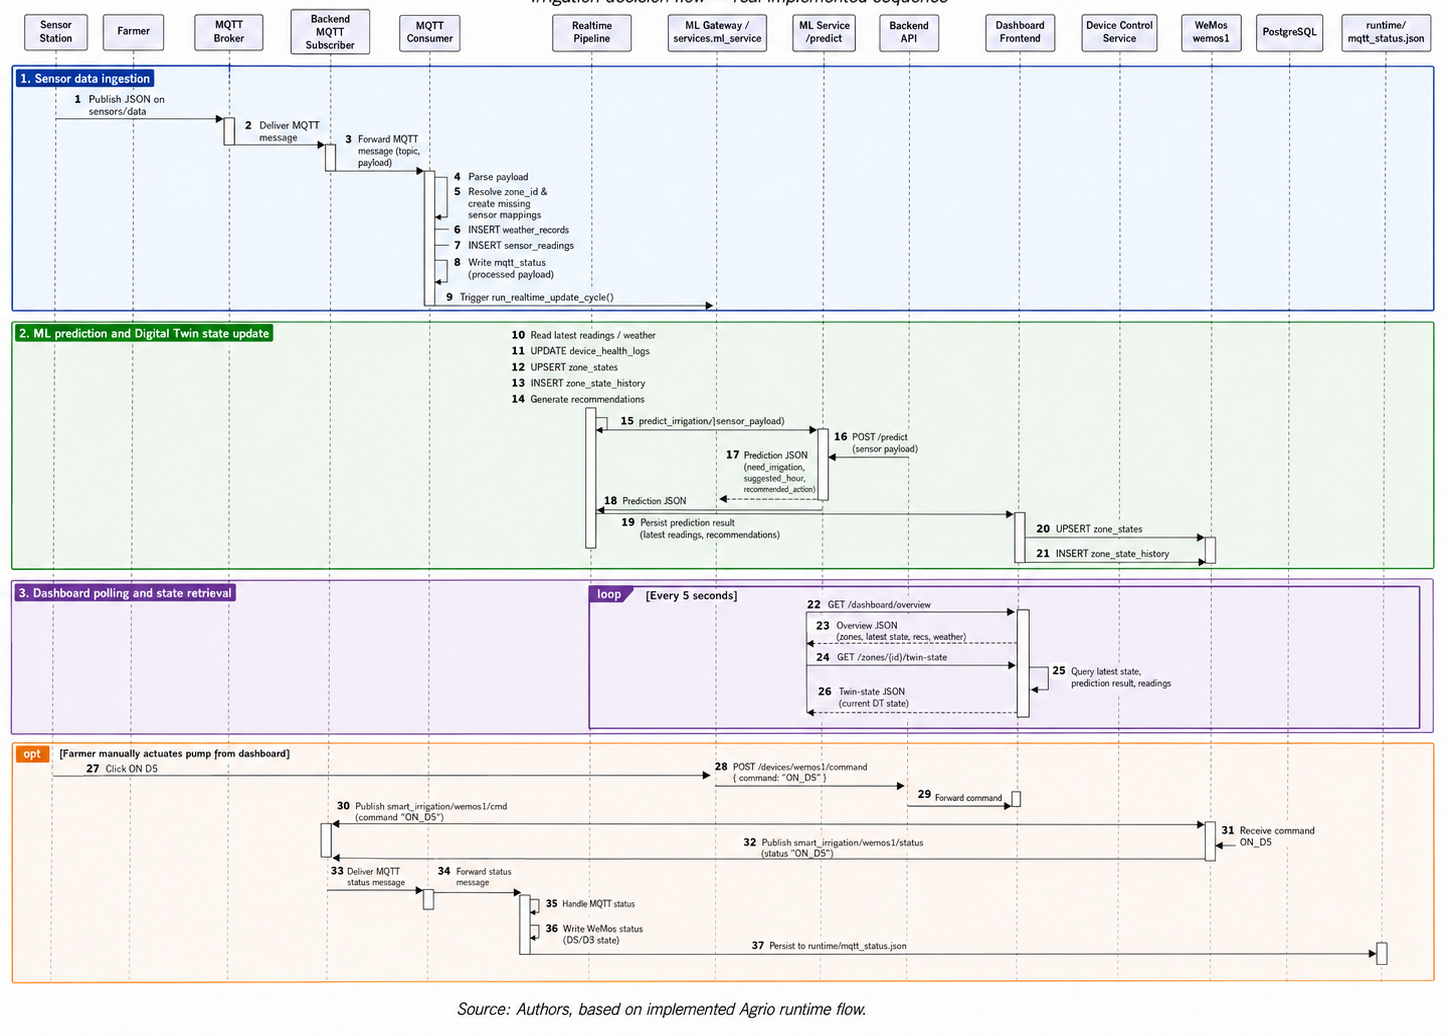
\includegraphics[width=0.92\textwidth,height=0.75\textheight,keepaspectratio]{figures/chapter_07/figure_7_runtime_sequence_clean.png}
    \caption{Sequence diagram of sensor ingestion, Digital Twin update, ML prediction, dashboard polling, and WeMos actuator command.}
    \label{fig:runtime_sequence_design}
\end{figure}

\noindent\textbf{Update note:} this sequence diagram should later be updated with a \texttt{mas-service} call between the Digital Twin/ML context and the final recommendation or validation step.

\section{Domain class diagrams}

The full domain model is too large to be readable as one figure. Therefore, it is split into four diagrams: agricultural domain, sensor/weather/forecast domain, Digital Twin/prediction/simulation domain, and decision/control domain. The complete class diagram is kept in Appendix~\ref{app:full_class_diagram}.

\begin{figure}[H]
    \centering
    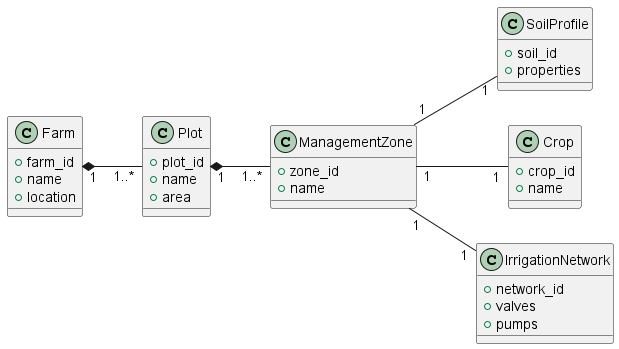
\includegraphics[width=\textwidth,height=0.85\textheight,keepaspectratio]{figures/chapter_05/fig_5-3.png}
    \caption{Agricultural domain class diagram representing farms, plots, zones, soil profiles, crops, and irrigation networks.}
    \label{fig:5-3-agricultural-domain-class-diagram-representing-farms-plots-zones-s}
\end{figure}

Figure~\ref{fig:5-3-agricultural-domain-class-diagram-representing-farms-plots-zones-s} describes the agricultural structure used by the platform. A \texttt{Farm} represents the global agricultural site. A \texttt{Plot} represents a physical cultivation area inside the farm. A \texttt{ManagementZone} represents the monitored irrigation unit where measurements, state updates, predictions, recommendations, and control decisions are attached. \texttt{SoilProfile} stores soil characteristics, while \texttt{Crop} stores crop information associated with the zone. \texttt{IrrigationNetwork} links a zone to the pump or valve infrastructure. The zone is central because most operational data in Table~\ref{tab:functional_requirements} must be interpreted at zone level before it can be used by the Digital Twin and the Chapter~\ref{chap:backend_database_iot} database implementation.

\begin{figure}[H]
    \centering
    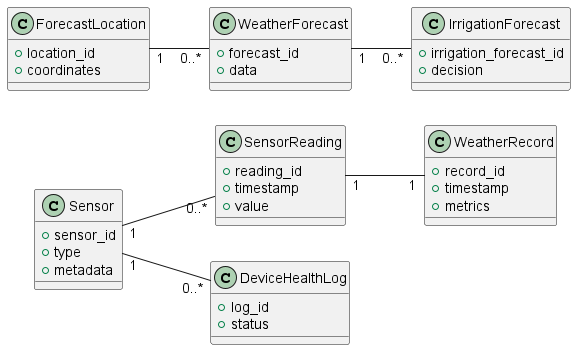
\includegraphics[width=\textwidth,height=0.85\textheight,keepaspectratio]{figures/chapter_05/fig_5-4.png}
    \caption{Sensor, weather, and forecasting data model used by the smart irrigation platform.}
    \label{fig:5-4-sensor-weather-and-forecasting-data-model-used-by-the-smart-irriga}
\end{figure}

Figure~\ref{fig:5-4-sensor-weather-and-forecasting-data-model-used-by-the-smart-irriga} connects real-time ingestion to planning. \texttt{Sensor} stores metadata for physical or virtual sensors. \texttt{SensorReading} stores timestamped measurements received from the ingestion pipeline. \texttt{WeatherRecord} stores environmental snapshots such as air temperature, humidity, rainfall, wind, and pressure. \texttt{DeviceHealthLog} records freshness and health status so stale measurements can be detected. \texttt{ForecastLocation}, \texttt{WeatherForecast}, and \texttt{IrrigationForecast} support weather-aware irrigation planning. Together, these classes allow the system to move from raw measurement to a forecast-aware decision context.

\begin{figure}[H]
    \centering
    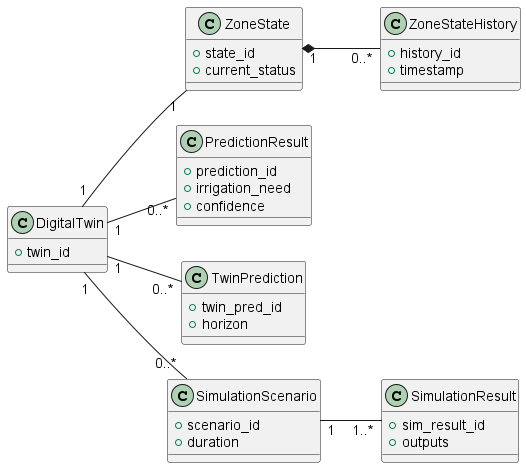
\includegraphics[width=\textwidth,height=0.85\textheight,keepaspectratio]{figures/chapter_05/fig_5-5.png}
    \caption{Digital Twin, prediction, and simulation data model.}
    \label{fig:5-5-digital-twin-prediction-and-simulation-data-model}
\end{figure}

\noindent\textbf{Update note:} this data model should later be updated to include MAS decision records or evidence snapshots if they are persisted in the final database schema.

Figure~\ref{fig:5-5-digital-twin-prediction-and-simulation-data-model} represents the virtual and intelligent part of the domain. \texttt{DigitalTwin} represents the virtual counterpart of a monitored zone. \texttt{ZoneState} stores the current synchronized state, while \texttt{ZoneStateHistory} preserves temporal evolution. \texttt{PredictionResult} stores ML outputs such as irrigation need, suggested hour, confidence, and fallback status. \texttt{TwinPrediction}, when used, stores longer-horizon outputs. \texttt{SimulationScenario} and \texttt{SimulationResult} store what-if inputs and outputs. This structure supports Digital Twin behavior because the platform can maintain state, preserve history, predict, and compare scenarios before actuation.

\begin{figure}[H]
    \centering
    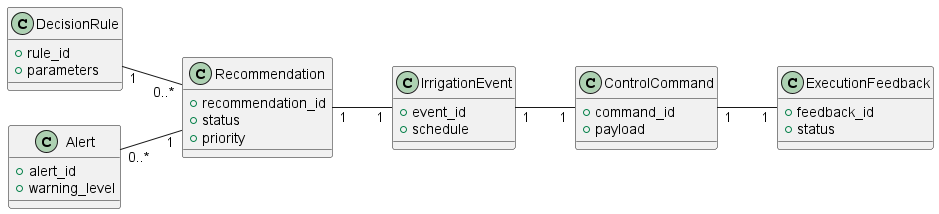
\includegraphics[width=\textwidth,height=0.85\textheight,keepaspectratio]{figures/chapter_05/fig_5-6.png}
    \caption{Decision, recommendation, scheduling, command, and feedback data model.}
    \label{fig:5-6-decision-recommendation-scheduling-command-and-feedback-data-model}
\end{figure}

\noindent\textbf{Update note:} this decision/control model should later be updated to show the MAS final decision, evidence bundle, warnings, risk level, and explanation fields when these artifacts are persisted.

Figure~\ref{fig:5-6-decision-recommendation-scheduling-command-and-feedback-data-model} closes the loop from recommendation to physical command. \texttt{Recommendation} stores suggested actions, priority, reason, confidence, and status. A validated-recommendation concept, when represented in the schema or workflow, captures human approval before execution. \texttt{IrrigationEvent} stores scheduled or actual irrigation. \texttt{ControlCommand} stores the command sent to the actuator, and \texttt{ExecutionFeedback} stores the actuator result or status. \texttt{Alert} and \texttt{DecisionRule} support warnings and rule logic. This design preserves traceability from a recommendation to a physical command and its feedback, which is one of the main requirements in Table~\ref{tab:functional_requirements}.

\section{Conclusion}

This chapter defined the requirements and design foundations of Agrio. It described the actors, functional requirements, non-functional requirements, constraints, use cases, workflow, runtime sequence, and domain class diagrams. The next chapter presents the global architecture that satisfies these requirements.
